\documentclass[english, a4paper,11pt]{article}
\usepackage[utf8]{inputenc}
\usepackage[T1]{fontenc,url} %url
\urlstyle{sf} %sf
\usepackage{babel,textcomp,csquotes, varioref,graphicx, gensymb}
% \usepackage[]{circuitikz}
\usepackage{tikz}
\usetikzlibrary{shapes,arrows}
\usepackage[backend=biber,style=numeric-comp, sortcites]{biblatex}

\bibliography{ref.bib} 

%opening
\title{Complete system testbech}
\author{Espen Klein Nilsen and \\Vegard Midtbøen}

\begin{document}

\maketitle

\section{Report contents}
This report contains a brief explanation of the different part in our project.   

\section{Structure}
The overall structure of the system is seen in Figure \ref{block_diagram}.

\tikzstyle{block} = [draw, fill=blue!20, rectangle, 
    minimum height=4em, minimum width=3em]
\tikzstyle{input} = [coordinate]
\tikzstyle{output} = [coordinate]
\tikzstyle{pinstyle} = [pin edge={to-,thin,black}]
\begin{figure}[!ht]
  \begin{tikzpicture}[auto, node distance=2cm,>=latex']
      % We start by placing the blocks
      \node [input, name=input] {};
      \node [block, right of=input, node distance=2cm] (sample_and_hold) {S\&H};
      \node [block, right of=sample_and_hold, node distance=4cm] (comparator) {Comparator};
      \node [block, right of=comparator, node distance=4cm] (sar_logic) {SAR Logic};
      
      % We draw an edge between the controller and system block to 
      % calculate the coordinate xsh(t). We need it to place the measurement block. 
      \draw [->] (sample_and_hold) -- node[name=xsh(t)] {$x_{sh}(t)$} (comparator);
      \draw [->] (comparator) -- node[name=xc(nT)] {$x_{c}(nT)$} (sar_logic);
      \node [block, below of=sar_logic, node distance=3cm] (dac){DAC};
      \node [output, right of=sar_logic, node distance=3cm] (output) {};
    
      % Once the nodes are placed, connecting them is easy. 
      \draw [draw,->] (input) -- node [name=xc(t)] {$x_{c}(t)$}(sample_and_hold);
      \draw [->] (sar_logic) -- node [name=digital_out] {Digital out}(output);
      \draw [->] (sar_logic) -- node [name=nbit] {N-bit} (dac);
      \draw [->] (dac) -| node [name=negfeedback, bend left] {Negative feedback}(comparator);     
  \end{tikzpicture}
  \caption{Block diagram}
  \label{block_diagram}
\end{figure}

\section{Schematic}  
\section*{Schematic: SAR\_system}
The SAR\_system is the complete schematic for the whole system. It consists of a sample and hold block, a comarator block, the SAR logic and the digital-to-analog converter block. Figure 
\ref{sar:system} shows the schematic that has been created.\\
\begin{figure}[!ht]
 \centering
   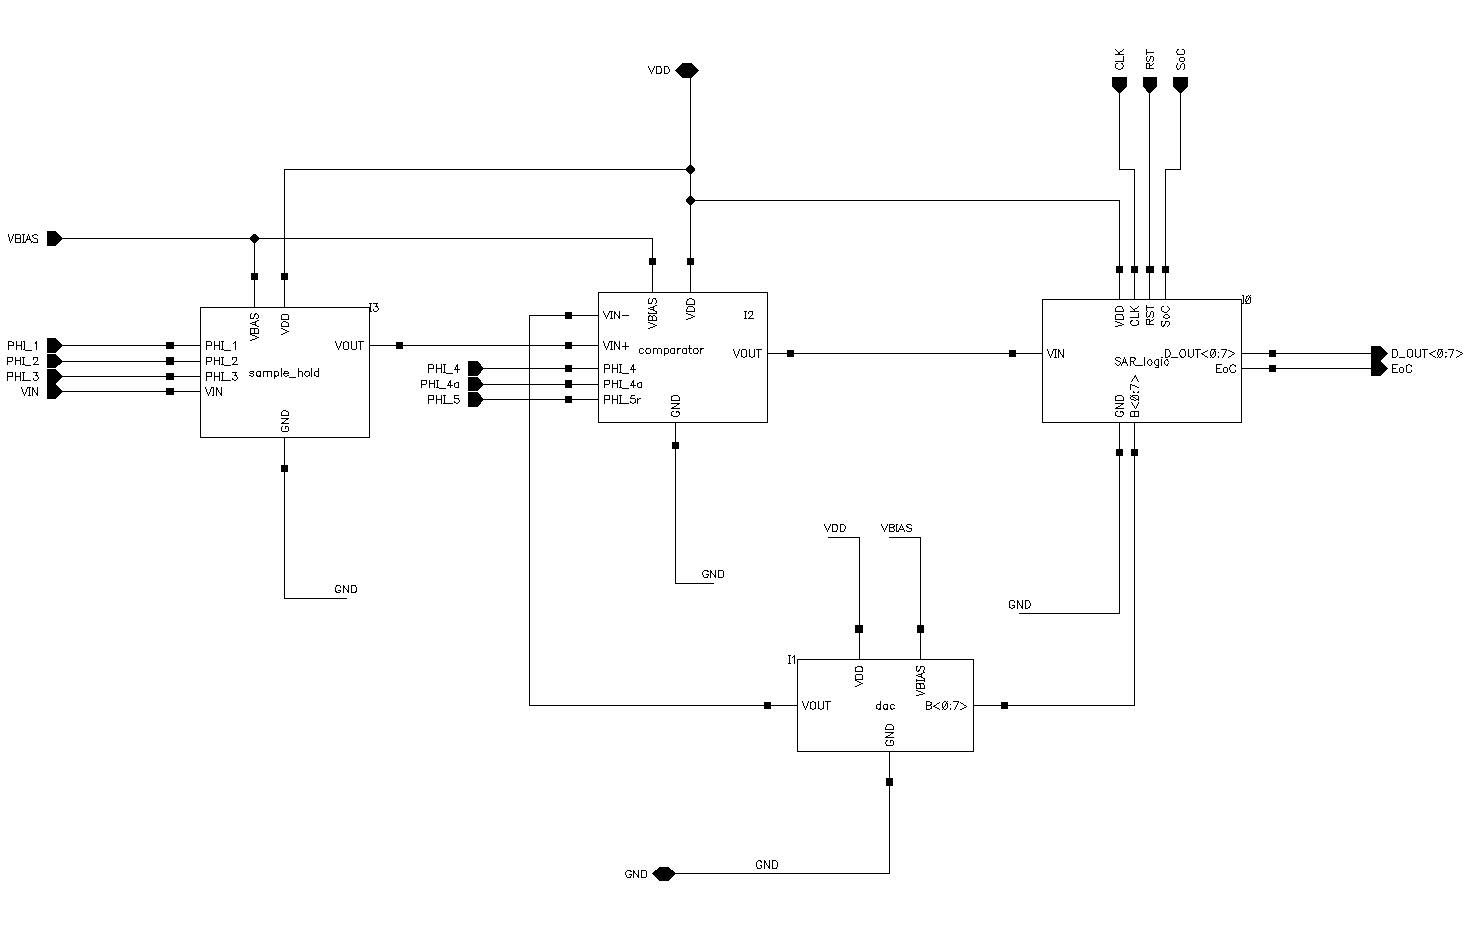
\includegraphics[width=\textwidth]{img/SAR_system}
   \caption{SAR\_system}
   \label{sar:system}
\end{figure}
\section*{Schematic: sample\_hold}
The sample and hold (S/H) is based on a circuit provided by R. Jacob Baker in the book CMOS Mixed-Signal Circut Design \cite{CMOS-baker}. The implementation is a single-ended S/H implementation. 
When $\phi_{1}$ and $\phi_{2}$ is high, $\phi_{3}$ is low, and the bottom plate of the hold capacitor is charged by the input signal, while the top plate is held to ground by the feedback around the 
op amp. When the $\phi_{2}$ is turned off, its charge will bee injected into the low impedance input, VIN, since the impedance looking into the left of the $\phi_{2}$ switch is large.\\
\\
This implementation has not yet beed tested, and may therefor be changed during the project.\\
\begin{figure}[!ht]
 \centering
   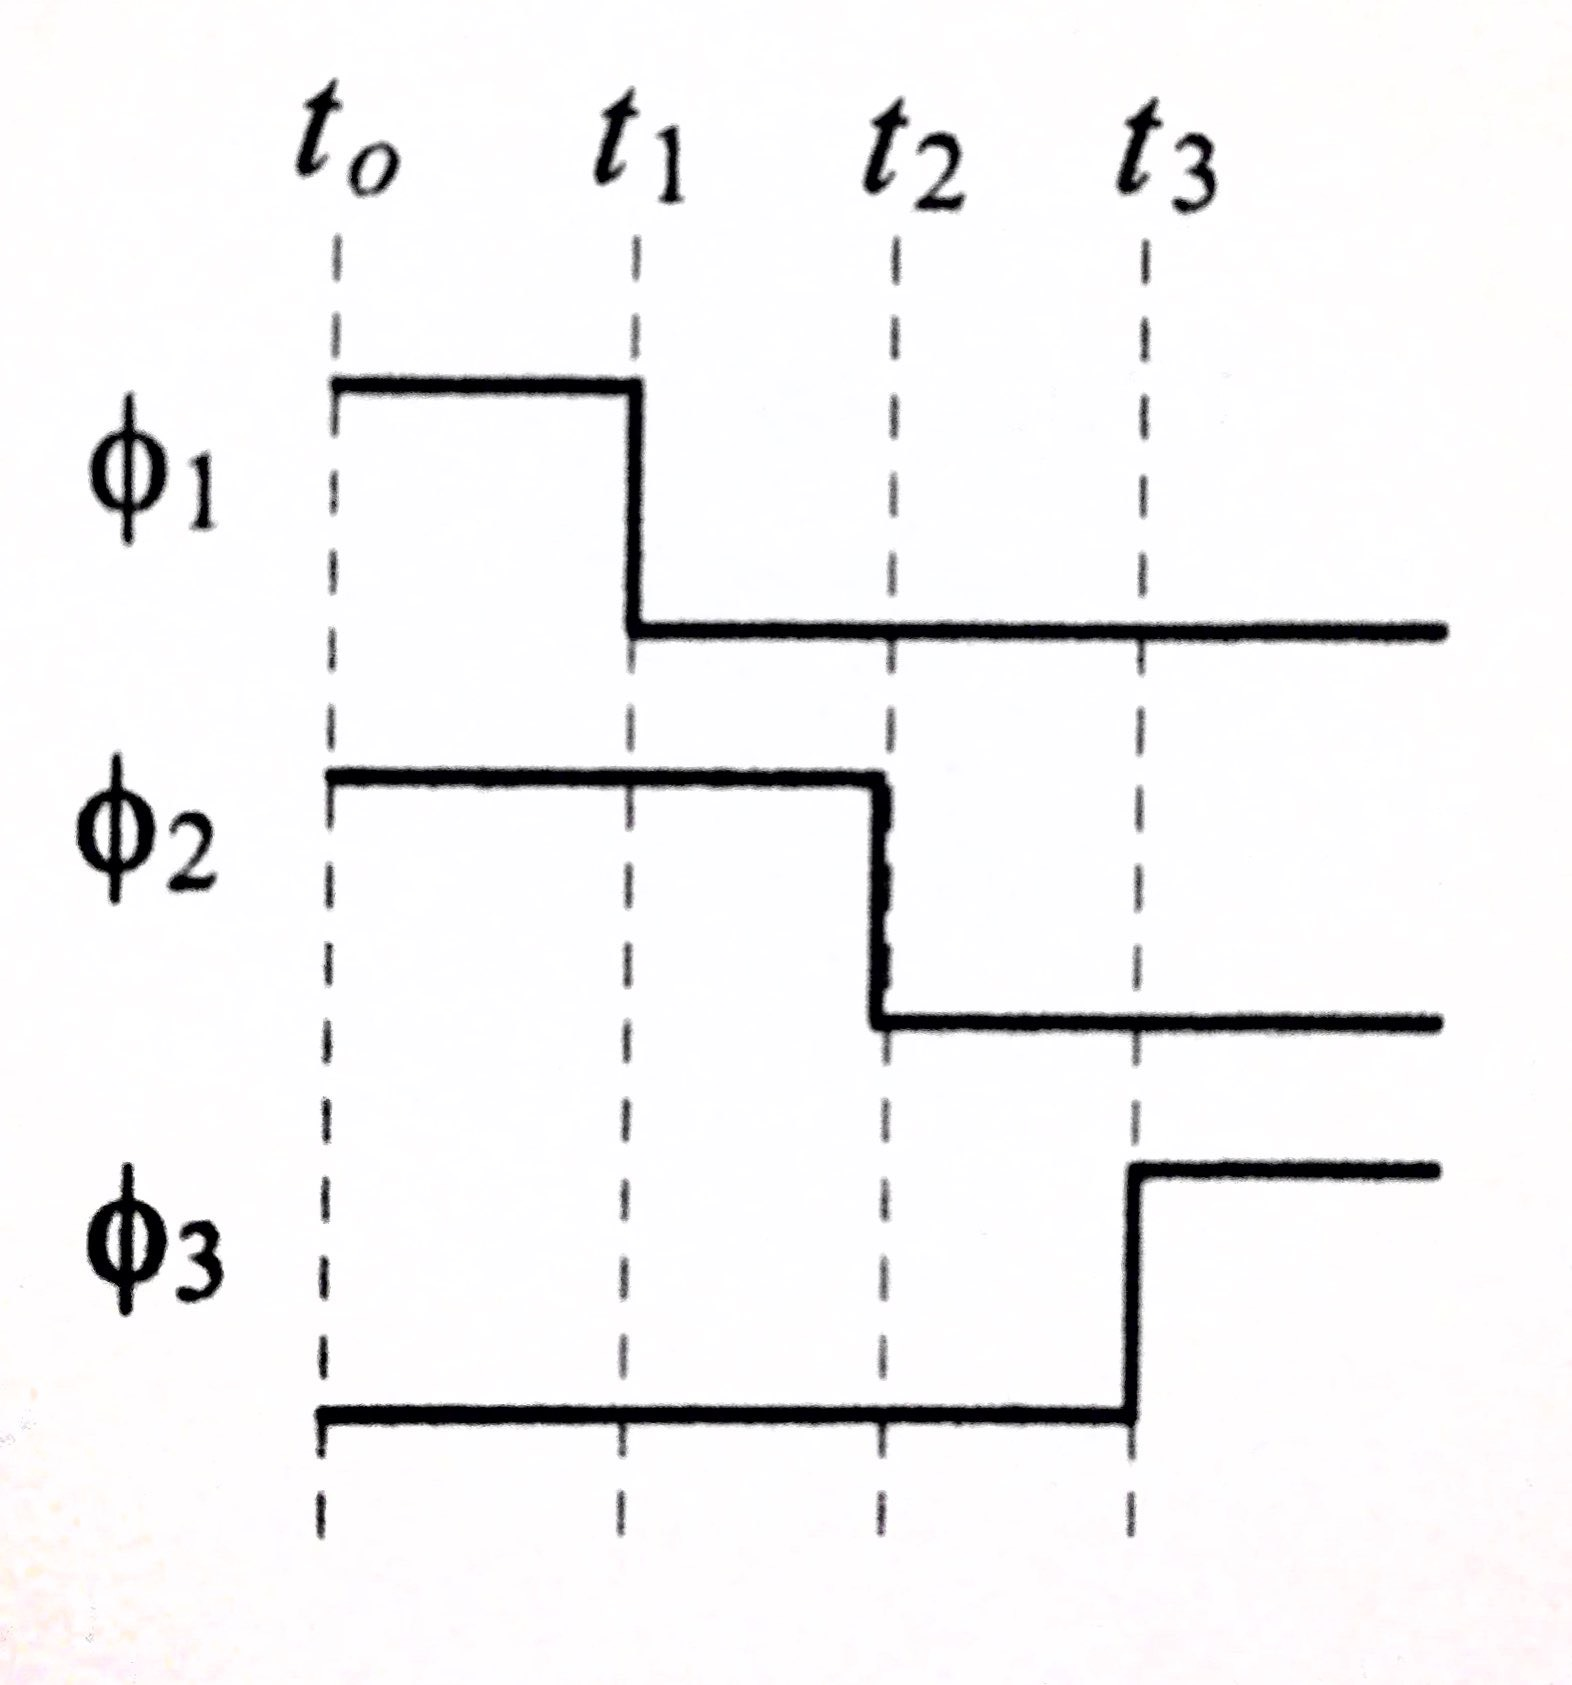
\includegraphics[width=0.3\textwidth]{img/timing_sample_hold.jpg}
   \caption{Single-ended S/H opartion \cite{CMOS-baker}}
   \label{timing}
\end{figure}
\begin{figure}[!ht]
 \centering
   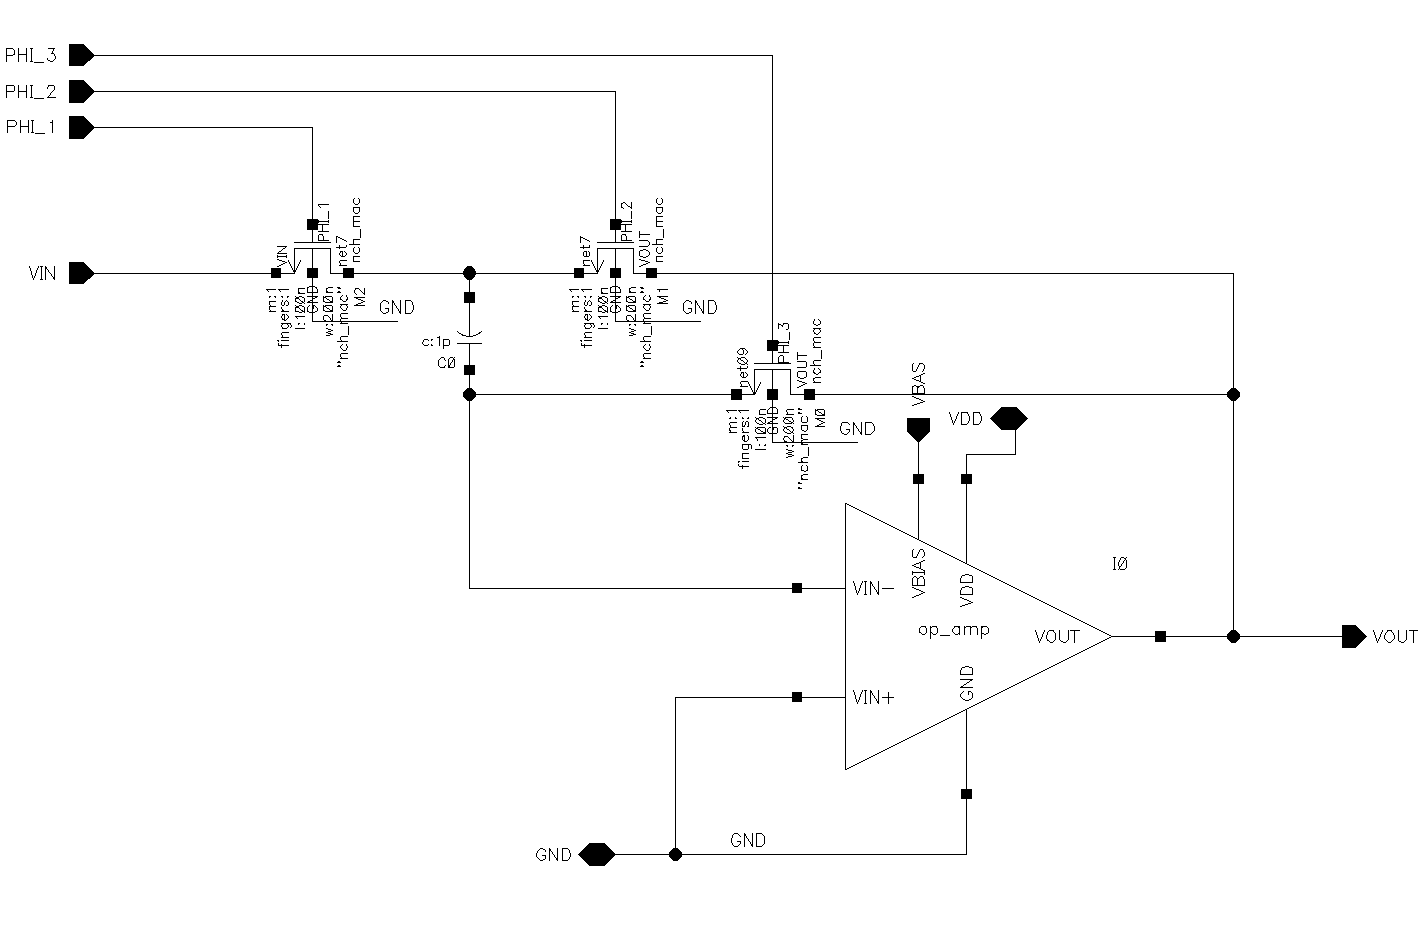
\includegraphics[width=\textwidth]{img/sample_hold}
   \caption{Sample and hold}
   \label{sample:hold}
\end{figure}
\section*{Schematic: comparator}
The design of the comparator 
\begin{figure}[!ht]
 \centering
   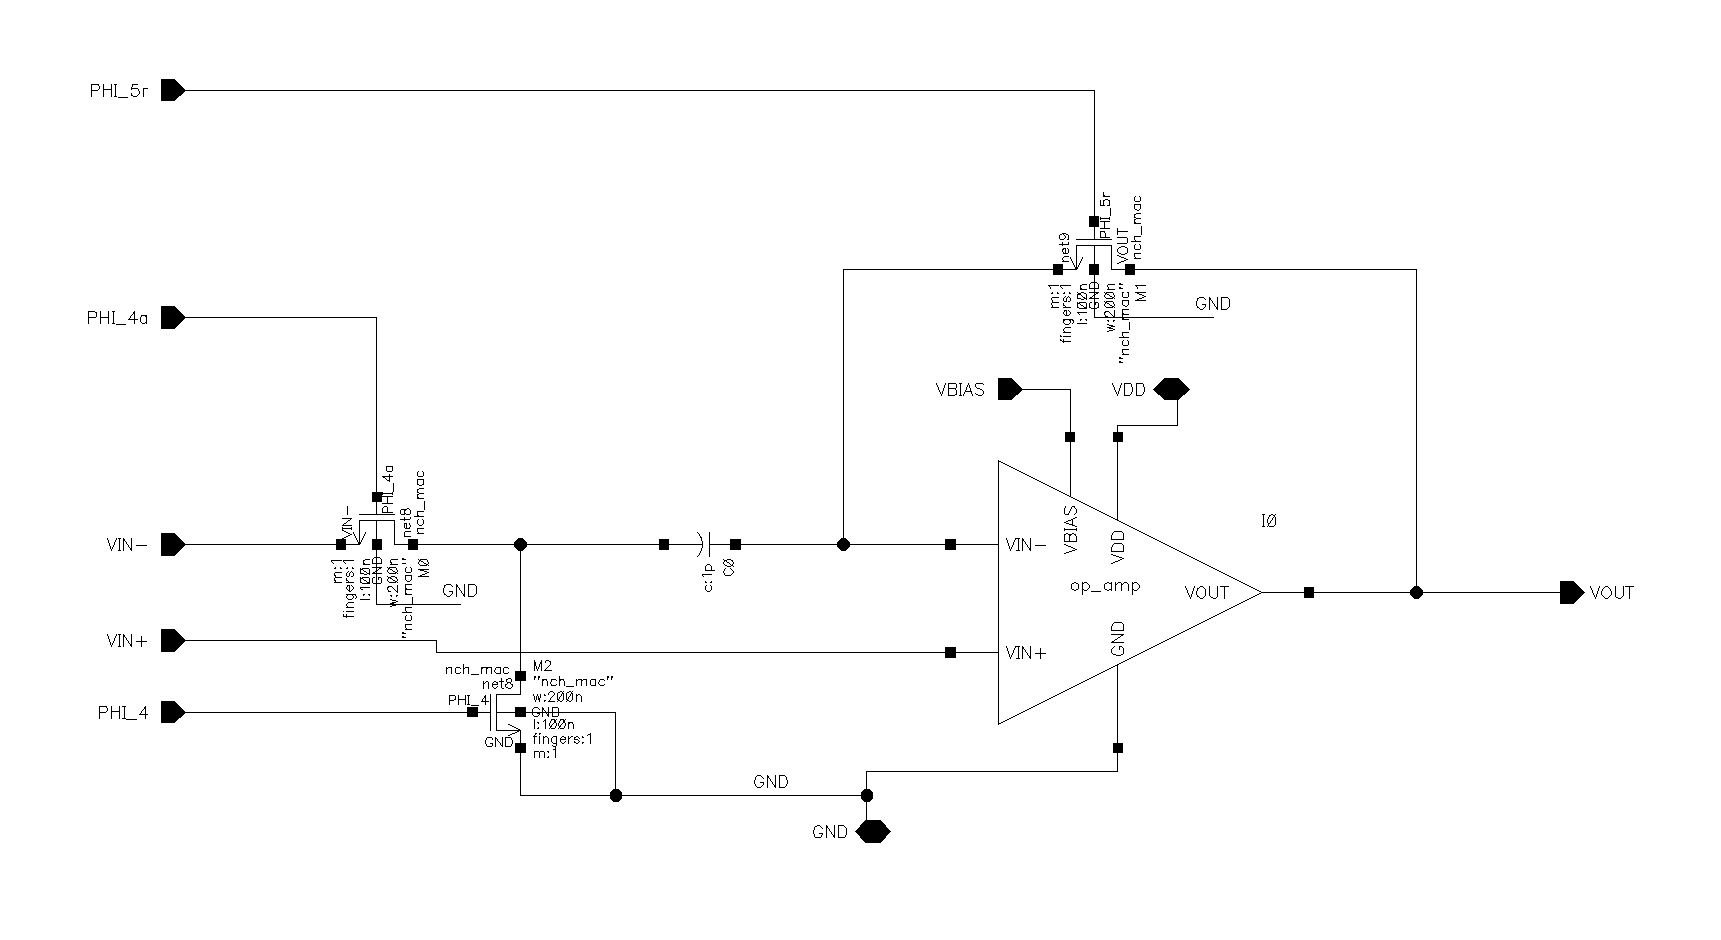
\includegraphics[width=\textwidth]{img/comparator}
   \caption{Comparator}
   \label{comparator}
\end{figure}
\section*{Schematic: SAR\_logic}
% \begin{figure}[!ht]
%  \centering
%    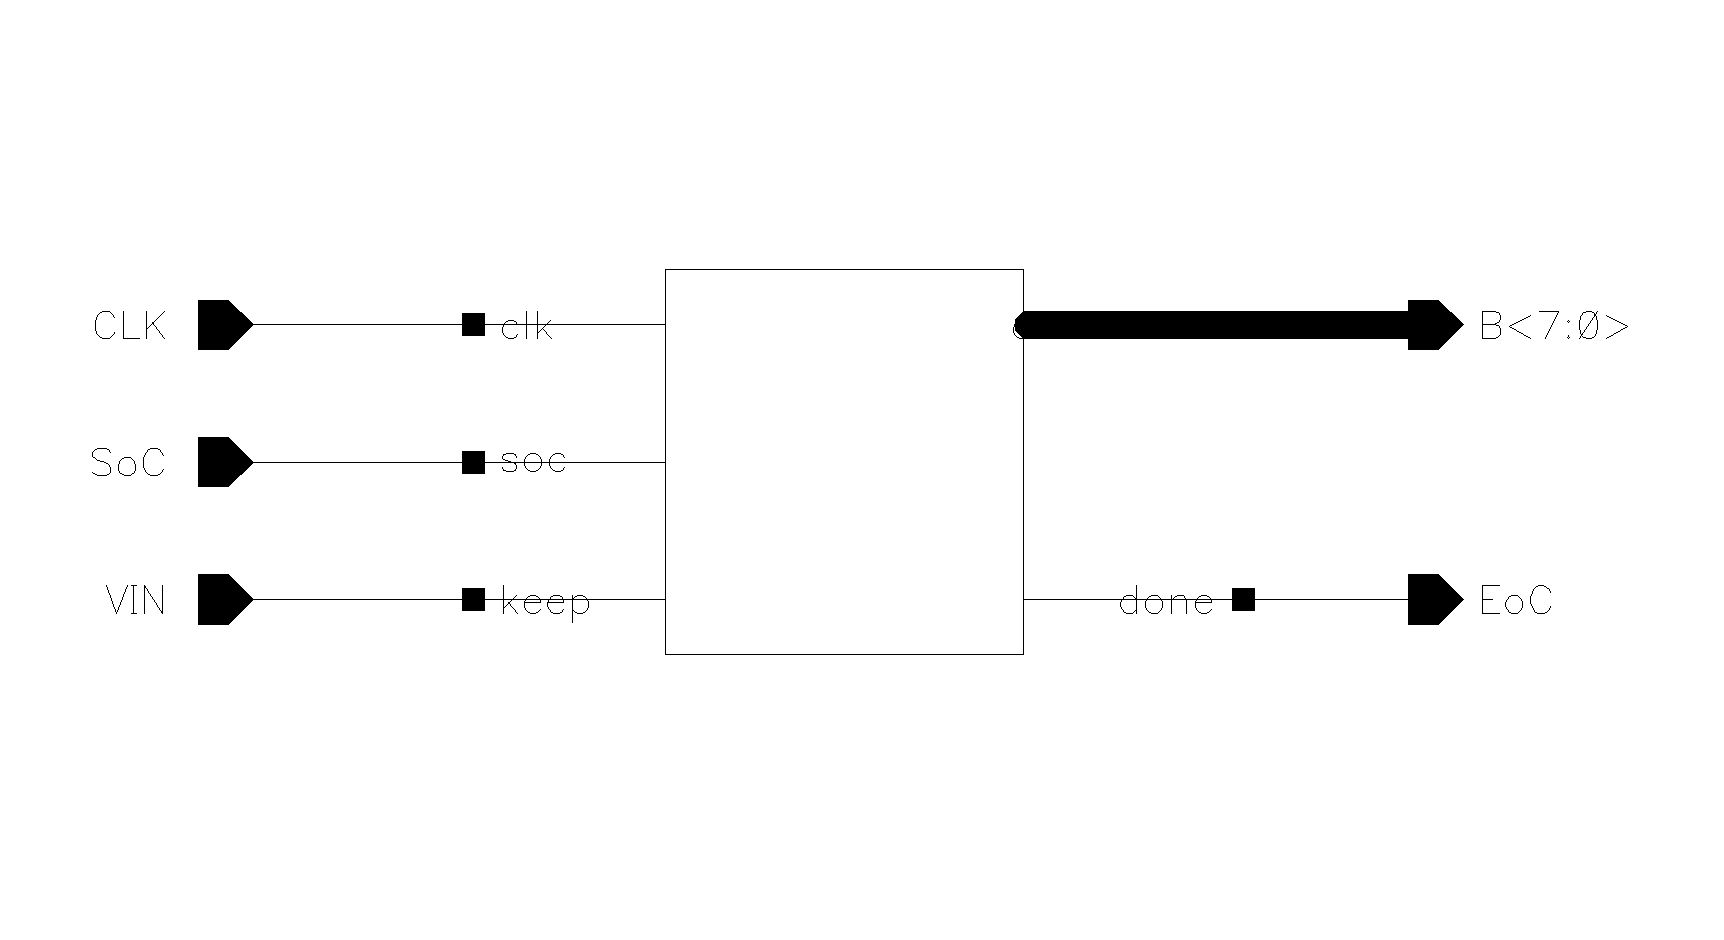
\includegraphics[width=0.4\textwidth]{img/SAR_logic}
%    \caption{Single-ended S/H opartion \cite{CMOS-baker}}
%    \label{timing}
% \end{figure}
\section*{Schematic: dac}
\begin{figure}[!ht]
 \centering
   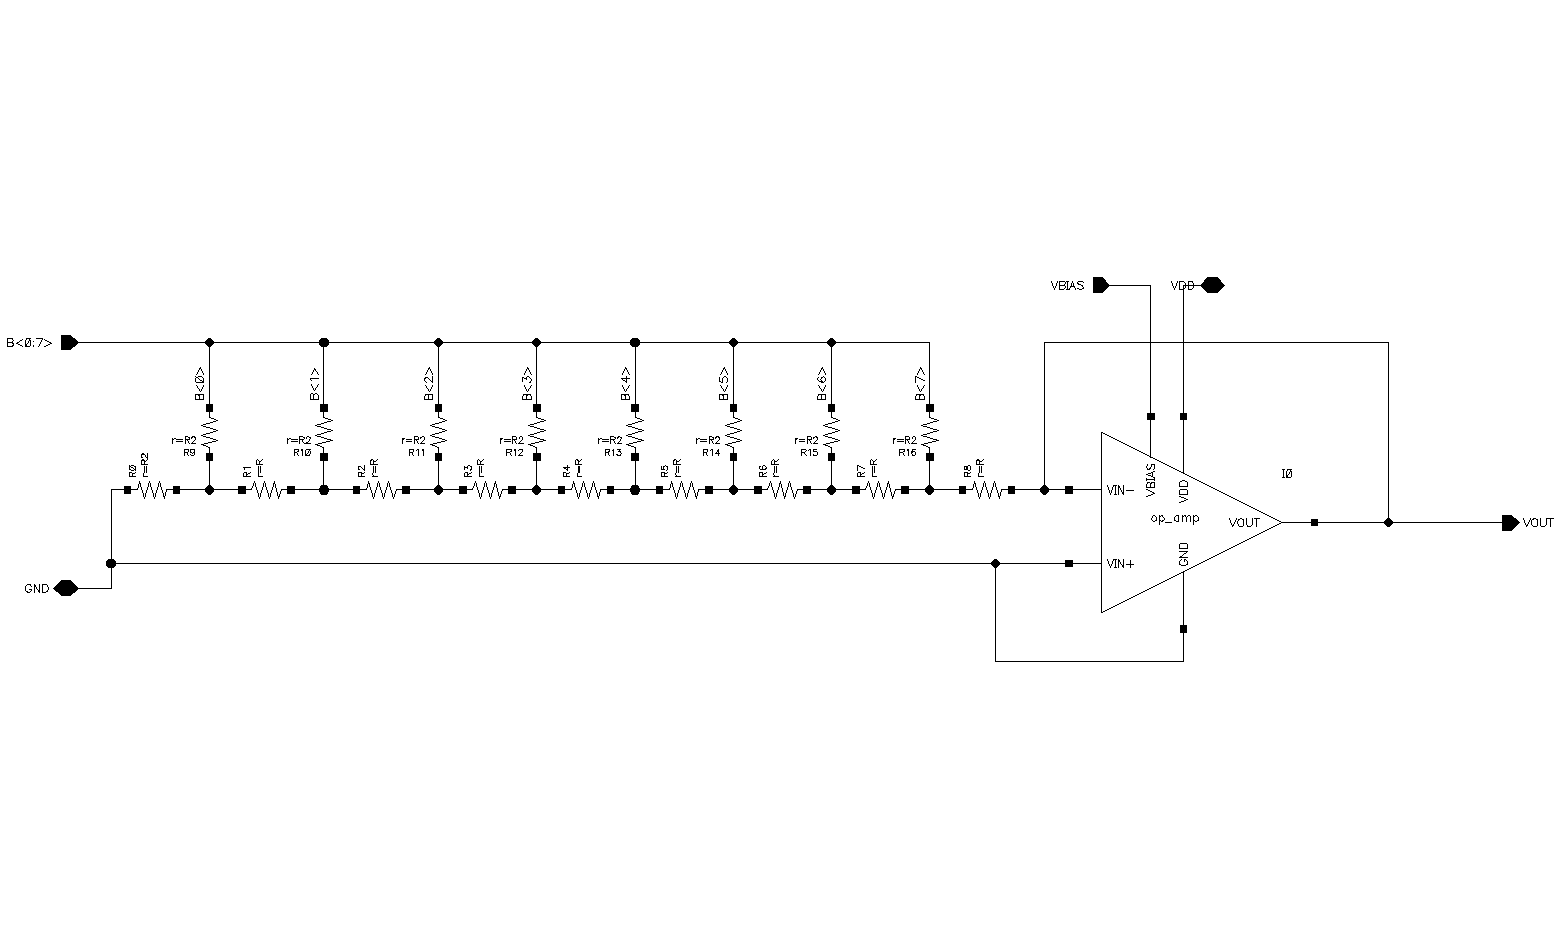
\includegraphics[width=\textwidth]{img/dac}
   \caption{DAC}
   \label{dac}
\end{figure}
\section*{Schematic: op\_amp}
\begin{figure}[!ht]
 \centering
   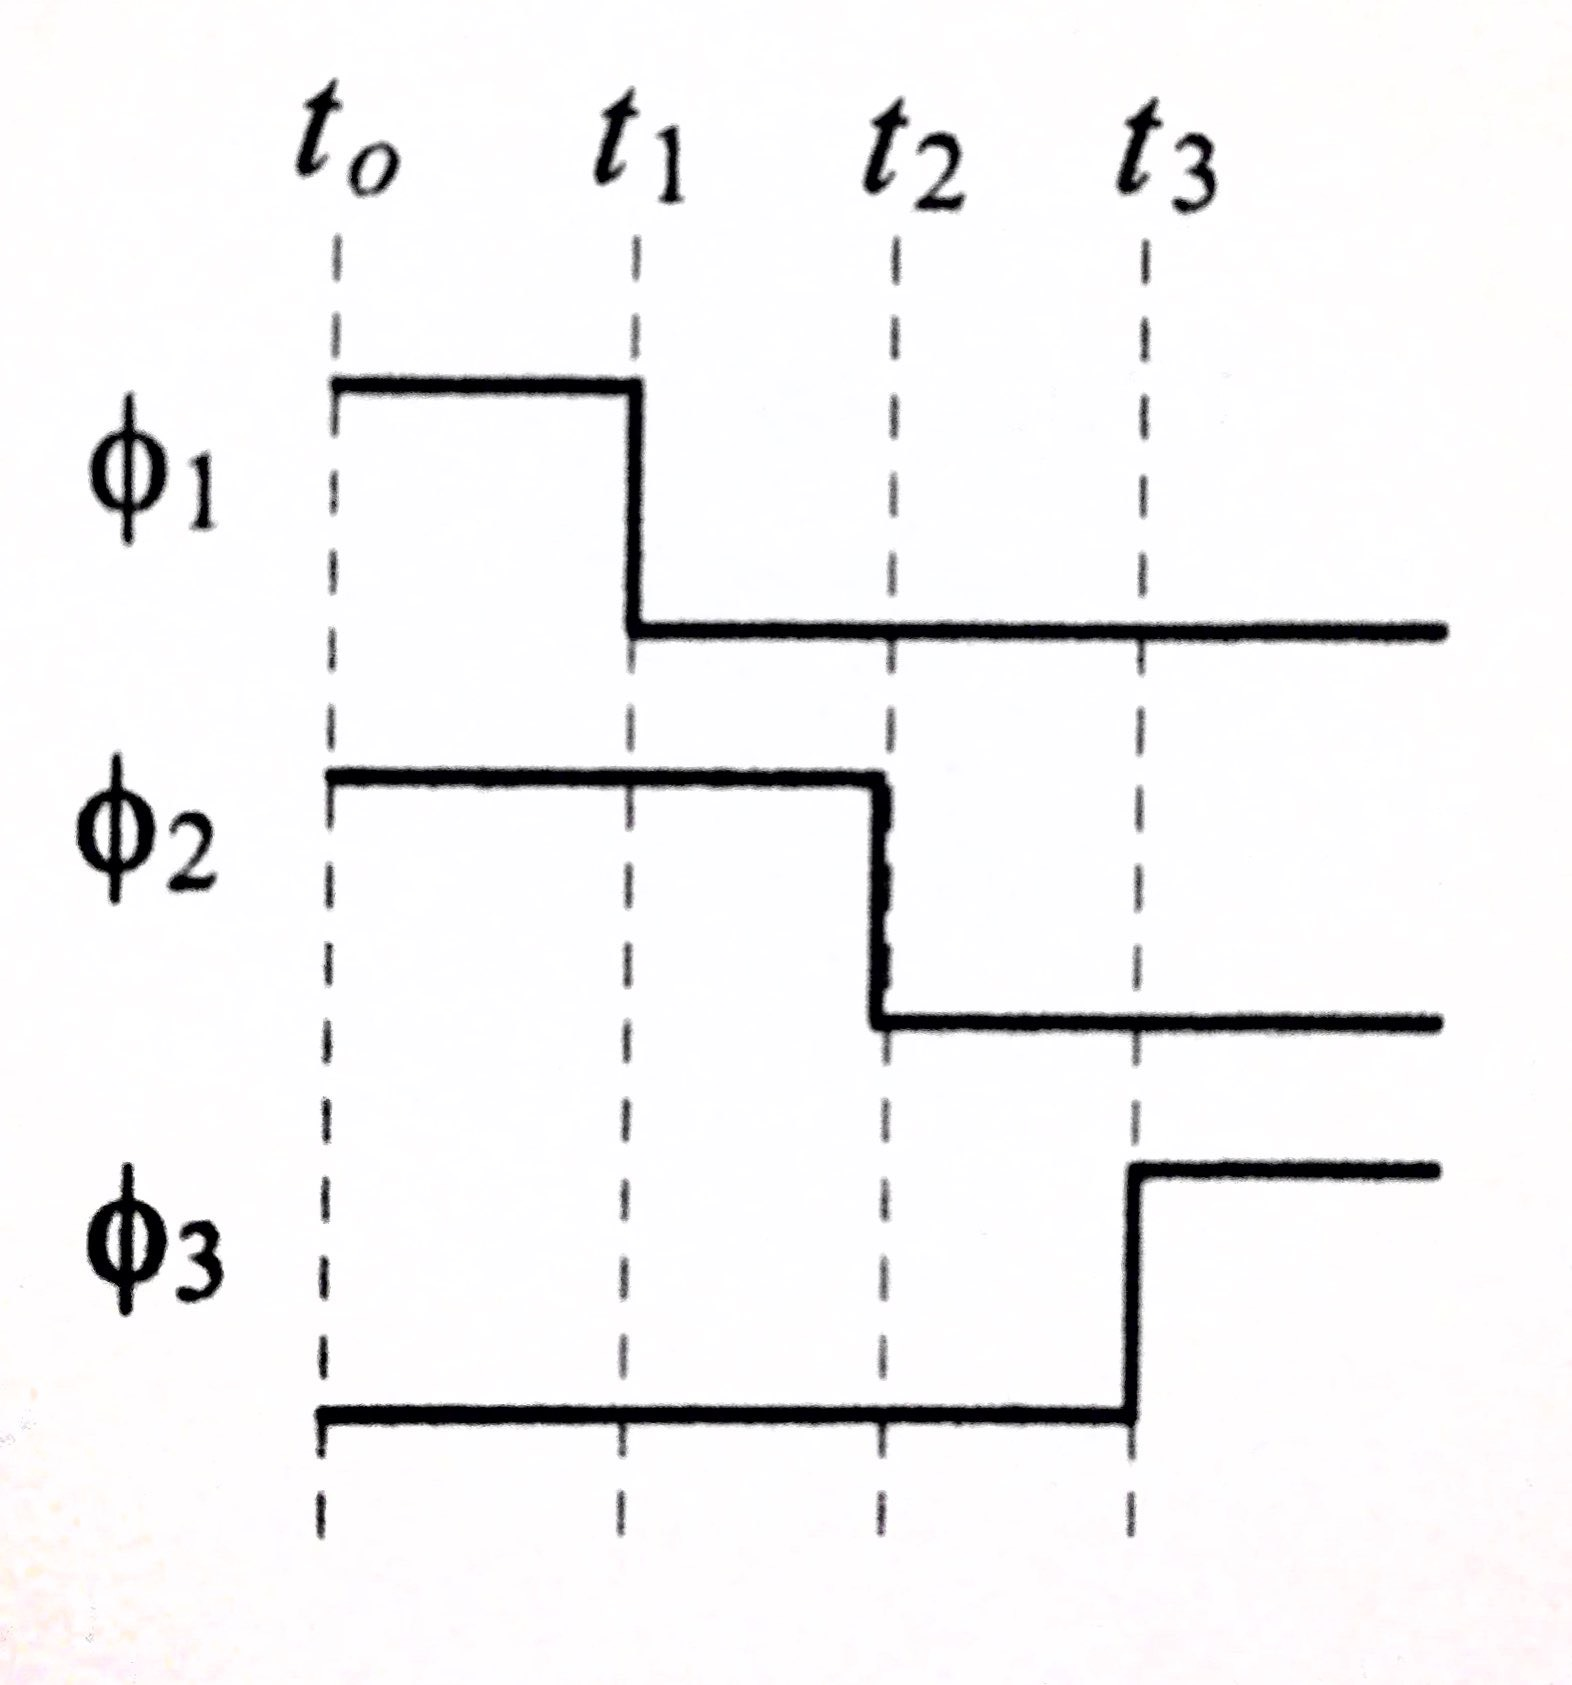
\includegraphics[width=0.4\textwidth]{img/timing_sample_hold.jpg}
   \caption{Single-ended S/H opartion \cite{CMOS-baker}}
   \label{timing}
\end{figure}

\section{Test bench}
\section*{Schematic: SIM\_system}
\begin{figure}[!ht]
 \centering
   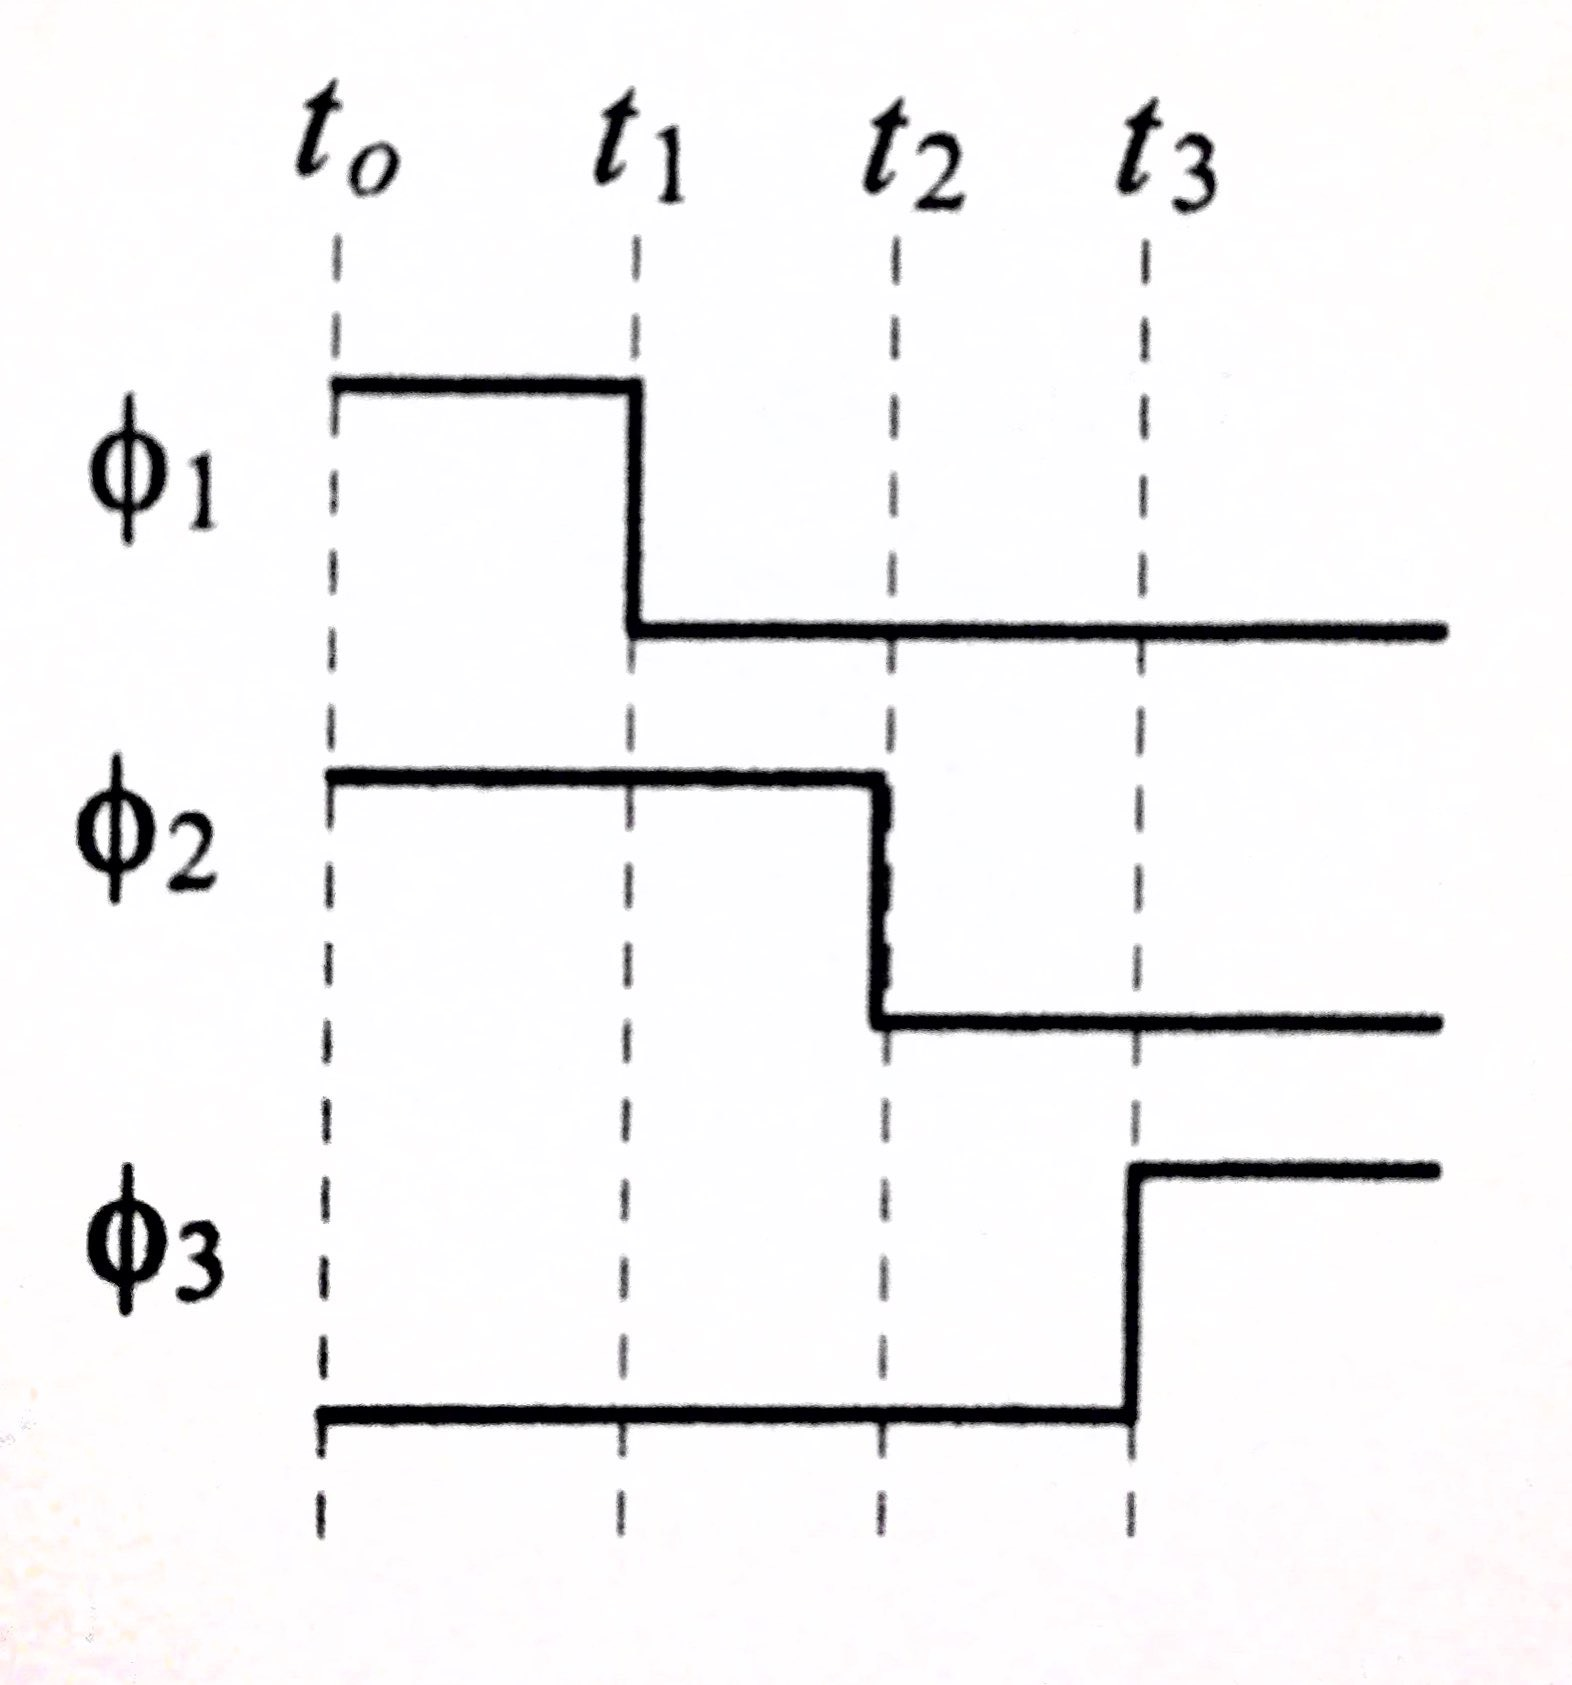
\includegraphics[width=0.4\textwidth]{img/timing_sample_hold.jpg}
   \caption{Single-ended S/H opartion \cite{CMOS-baker}}
   \label{timing}
\end{figure}
\section*{Schematic: SIM\_sample\_hold}
\begin{figure}[!ht]
 \centering
   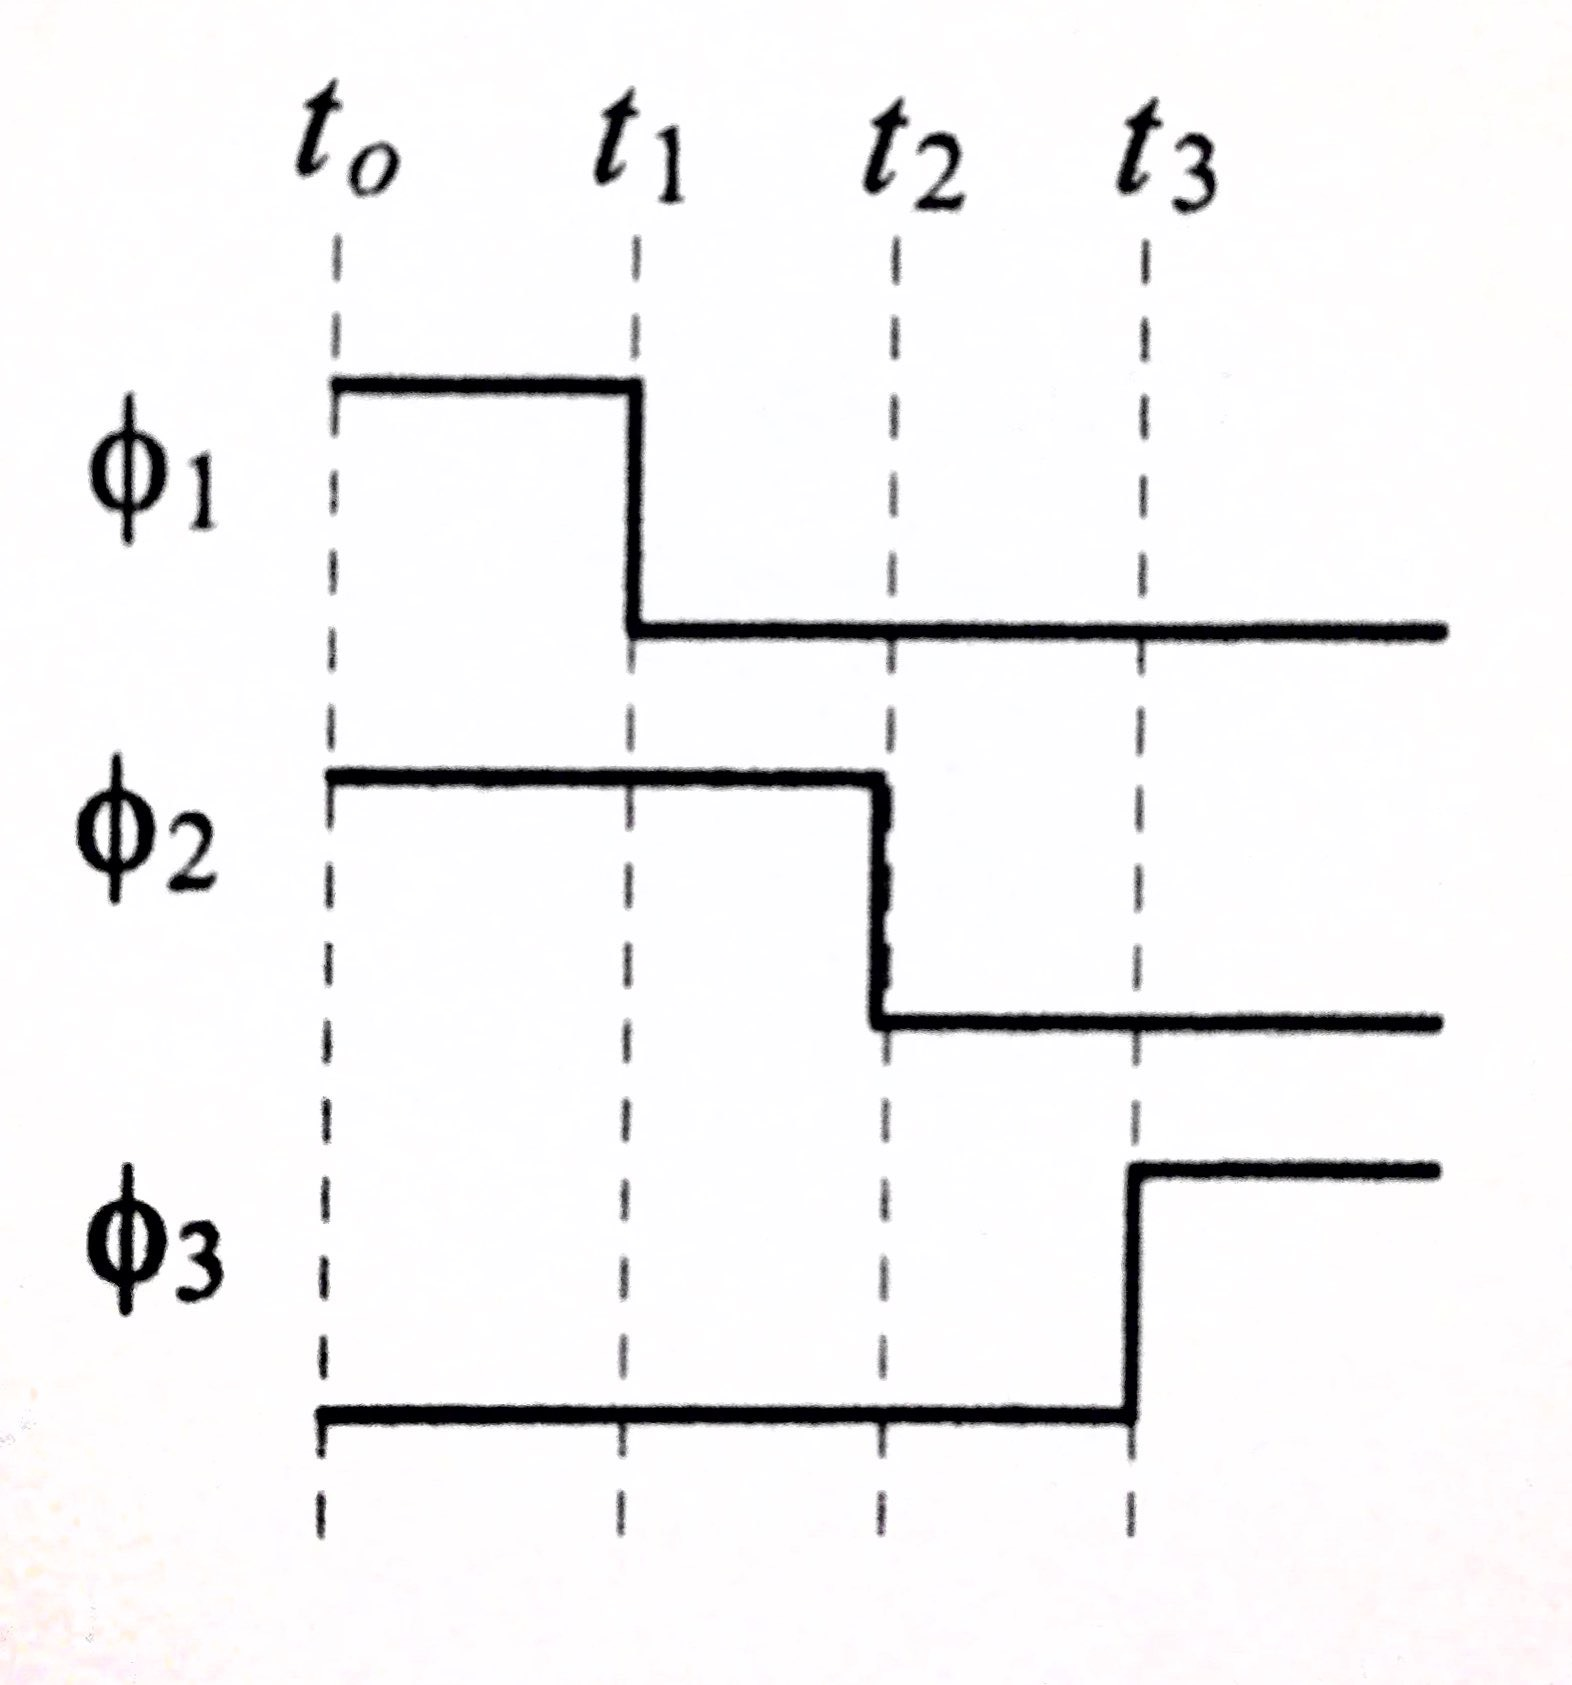
\includegraphics[width=0.4\textwidth]{img/timing_sample_hold.jpg}
   \caption{Single-ended S/H opartion \cite{CMOS-baker}}
   \label{timing}
\end{figure}
\section*{Schematic: SIM\_comparator}
\begin{figure}[!ht]
 \centering
   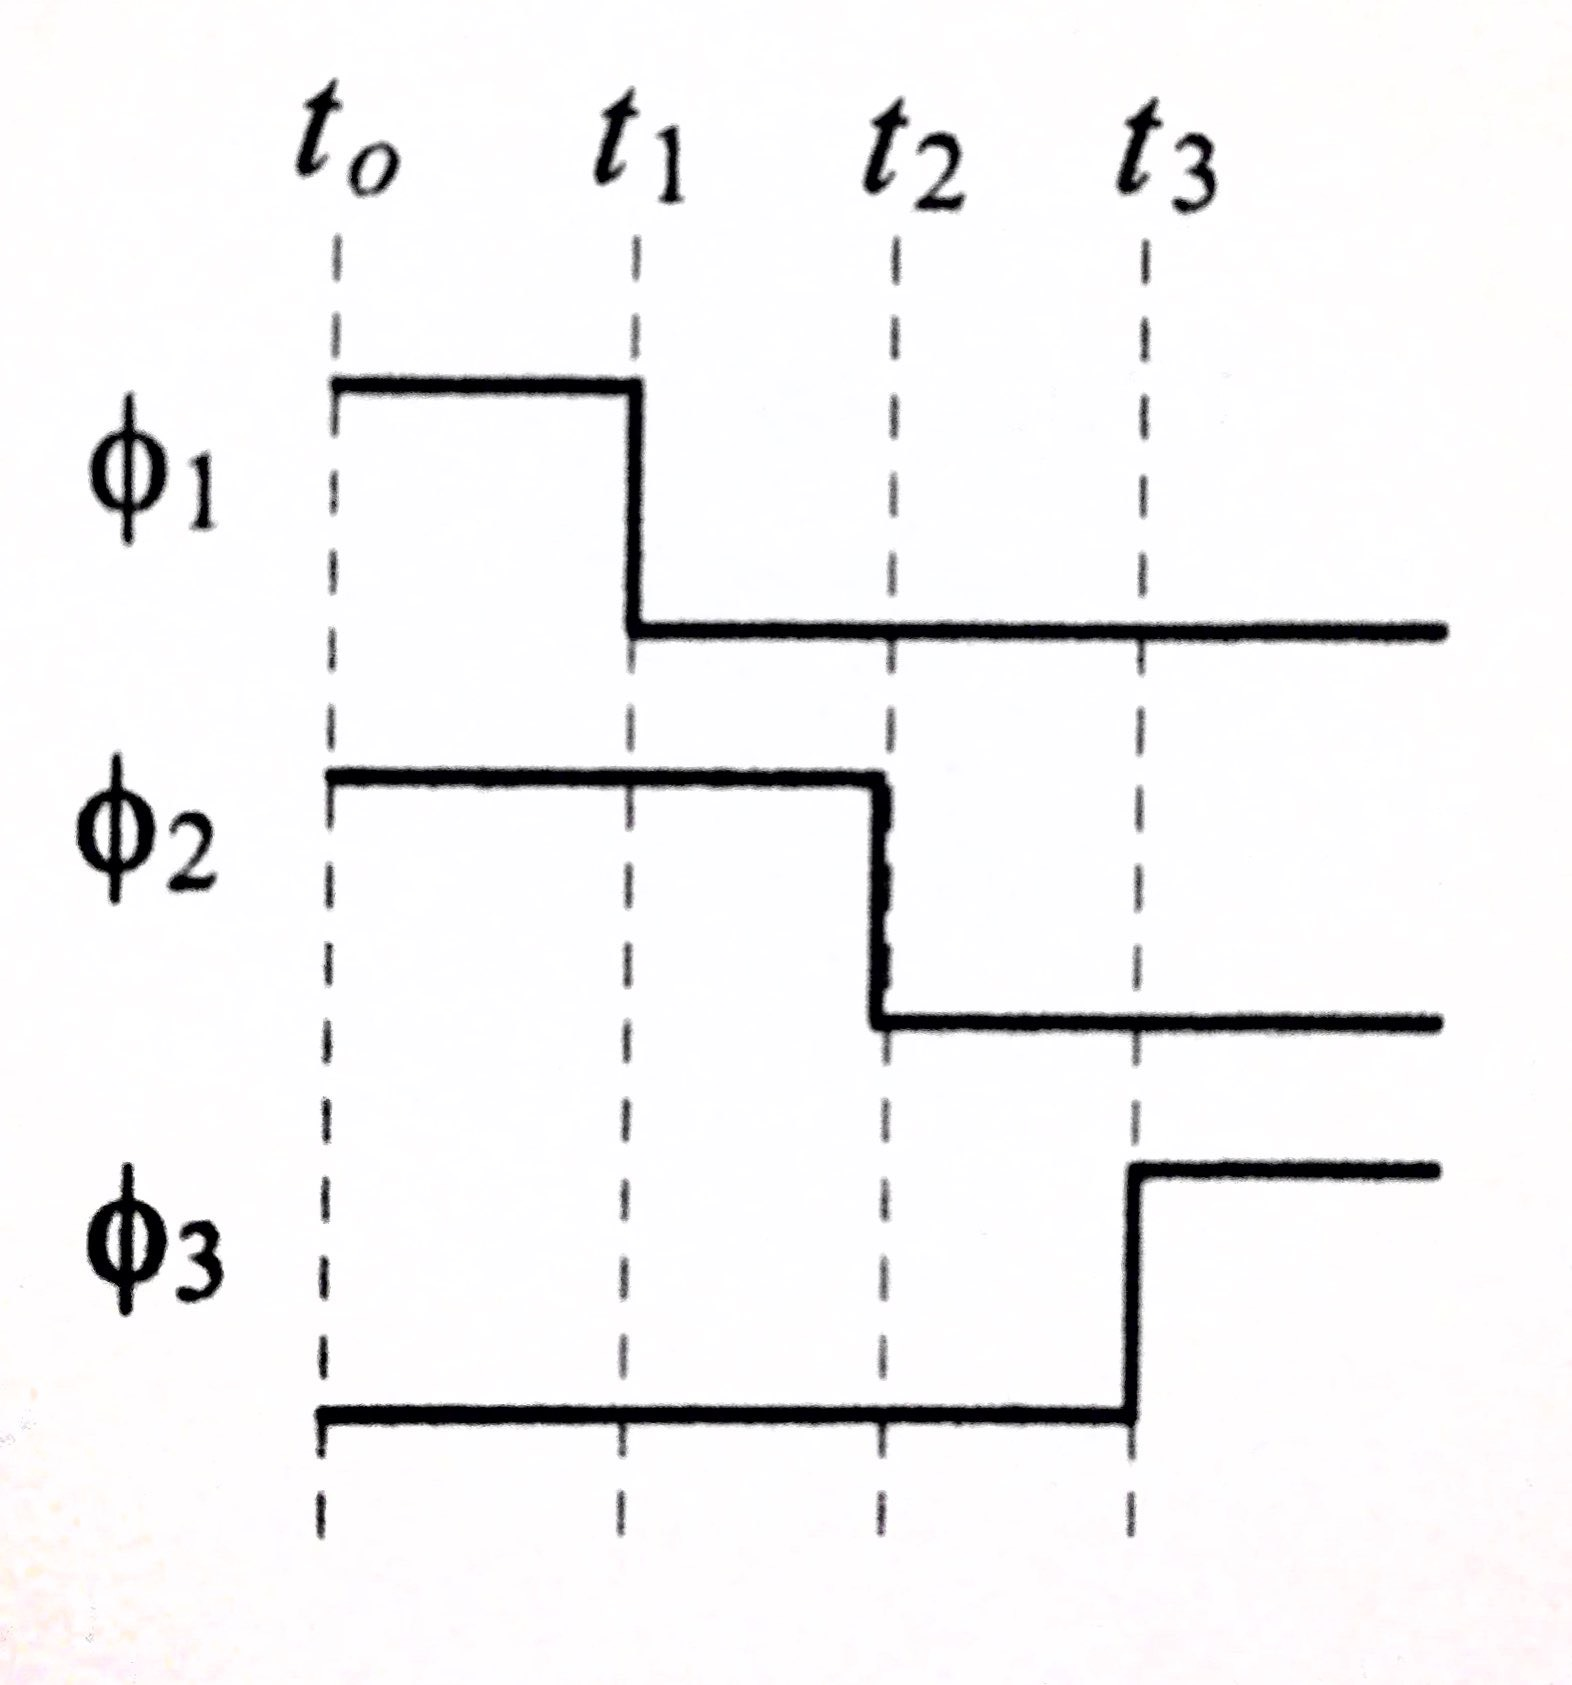
\includegraphics[width=0.4\textwidth]{img/timing_sample_hold.jpg}
   \caption{Single-ended S/H opartion \cite{CMOS-baker}}
   \label{timing}
\end{figure}
\section*{Schematic: SIM\_SAR\_logic}
\begin{figure}[!ht]
 \centering
   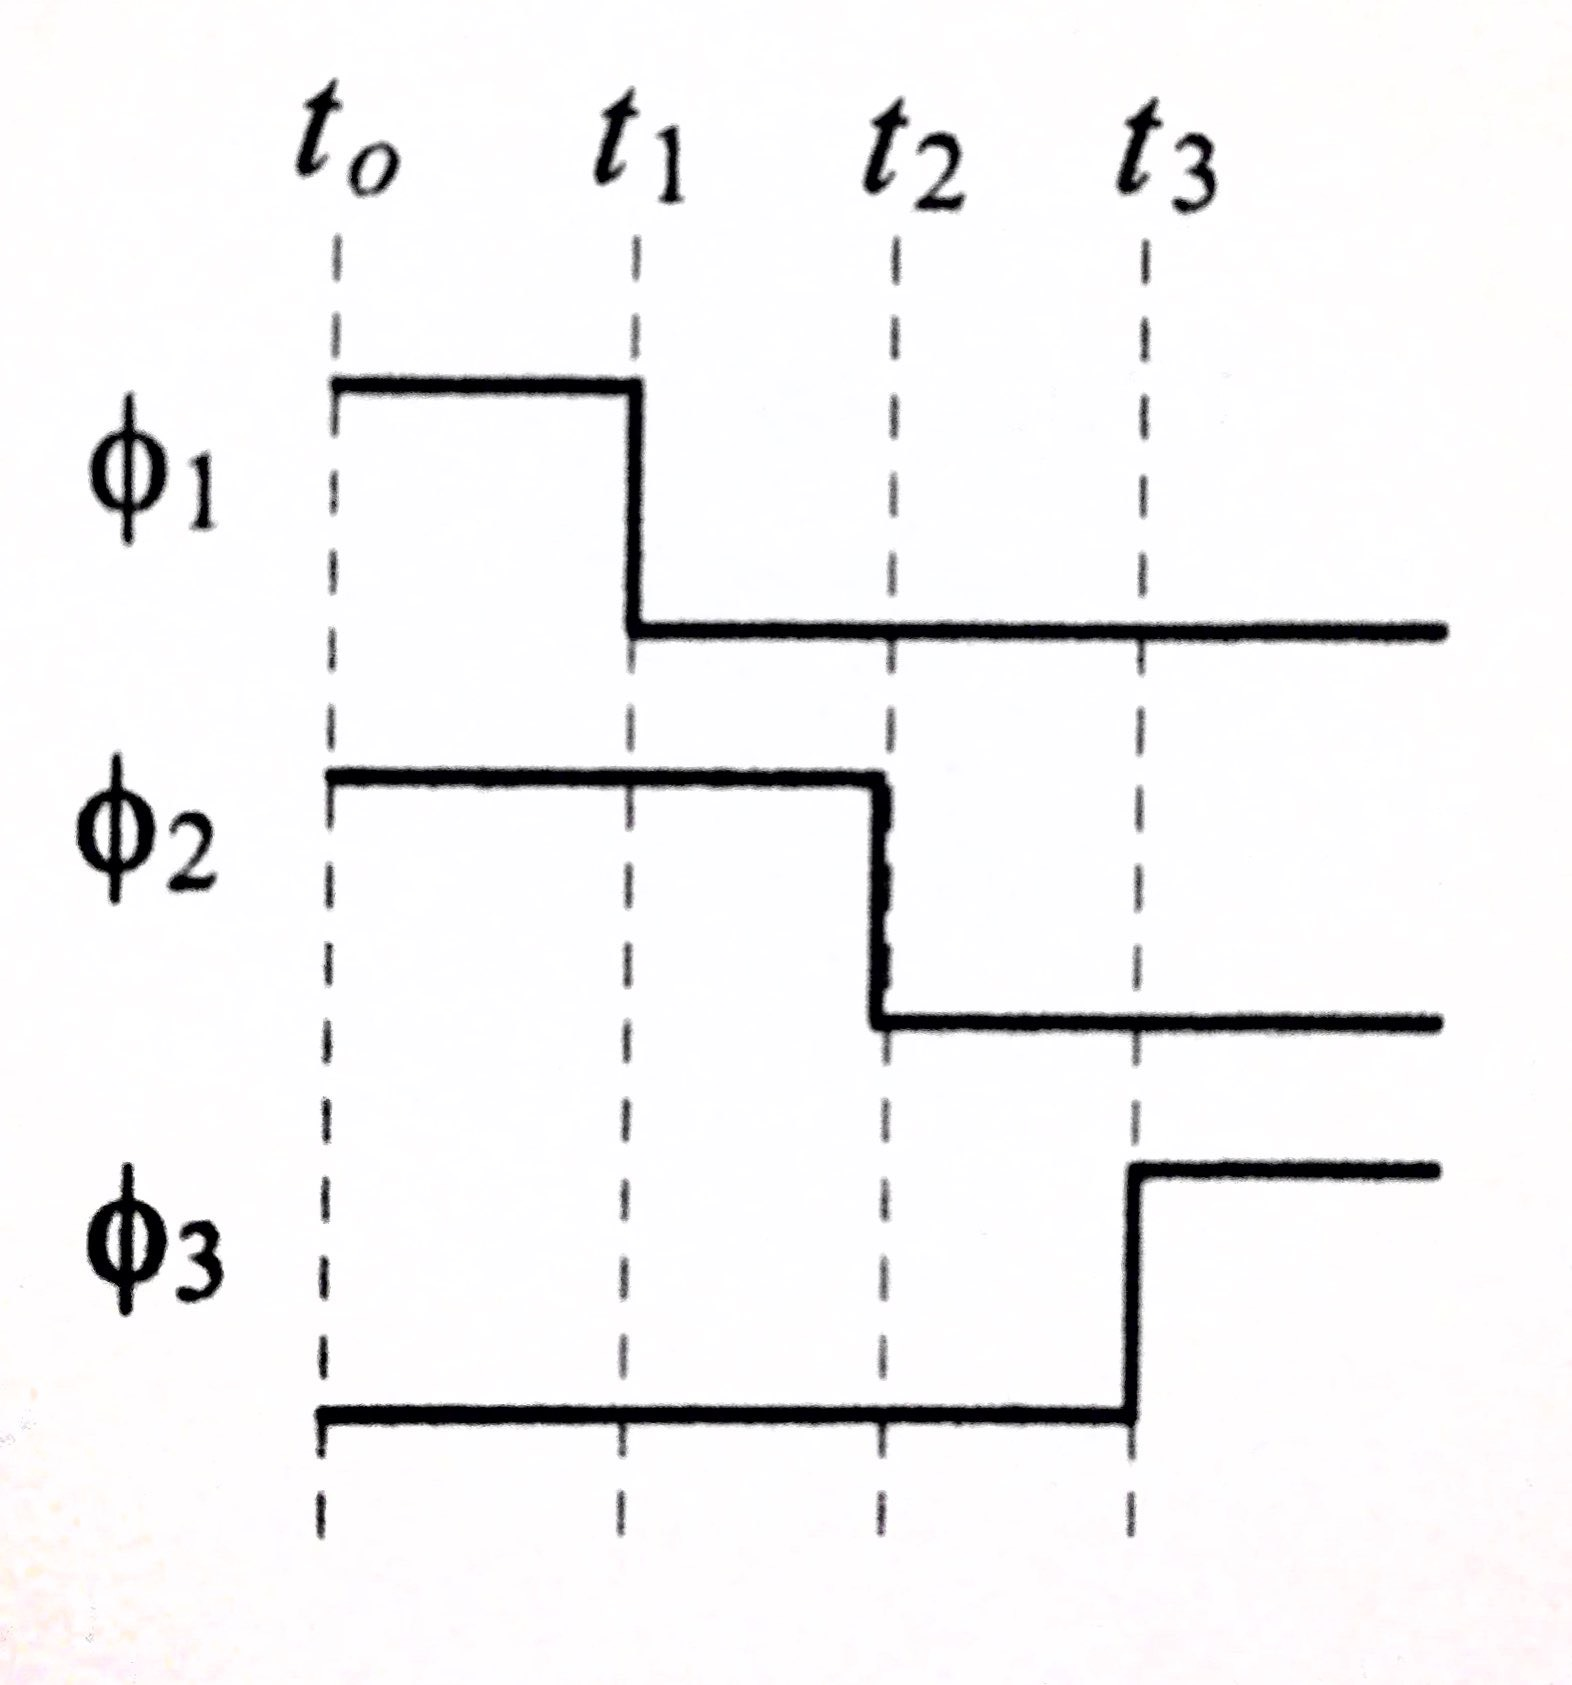
\includegraphics[width=0.4\textwidth]{img/timing_sample_hold.jpg}
   \caption{Single-ended S/H opartion \cite{CMOS-baker}}
   \label{timing}
\end{figure}
\section*{Schematic: SIM\_dac}
\begin{figure}[!ht]
 \centering
   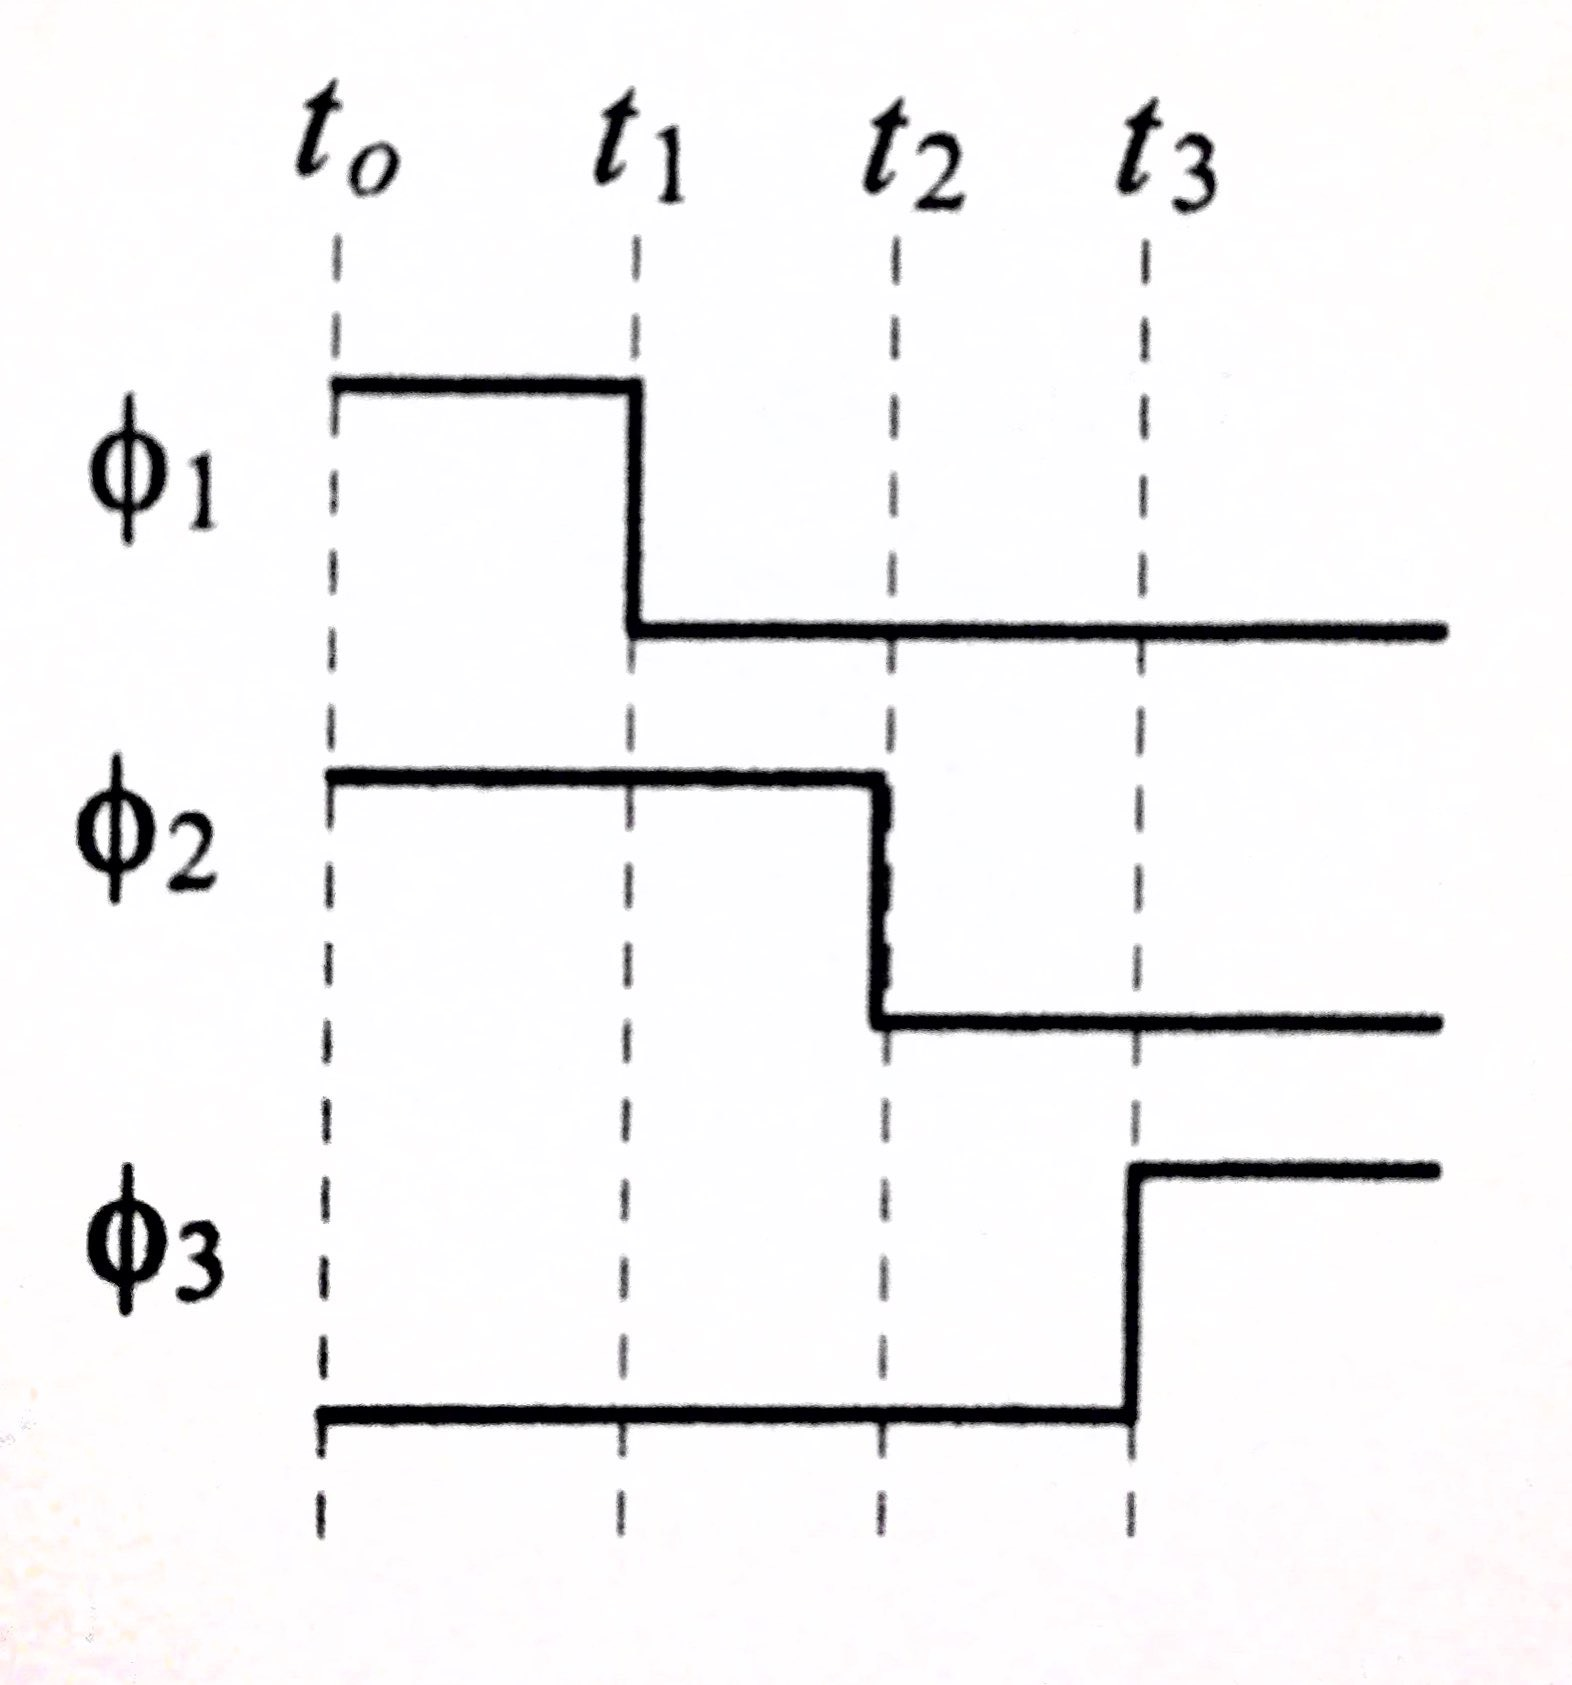
\includegraphics[width=0.4\textwidth]{img/timing_sample_hold.jpg}
   \caption{Single-ended S/H opartion \cite{CMOS-baker}}
   \label{timing}
\end{figure}
\section*{Schematic: SIM\_op\_amp}
\begin{figure}[!ht]
 \centering
   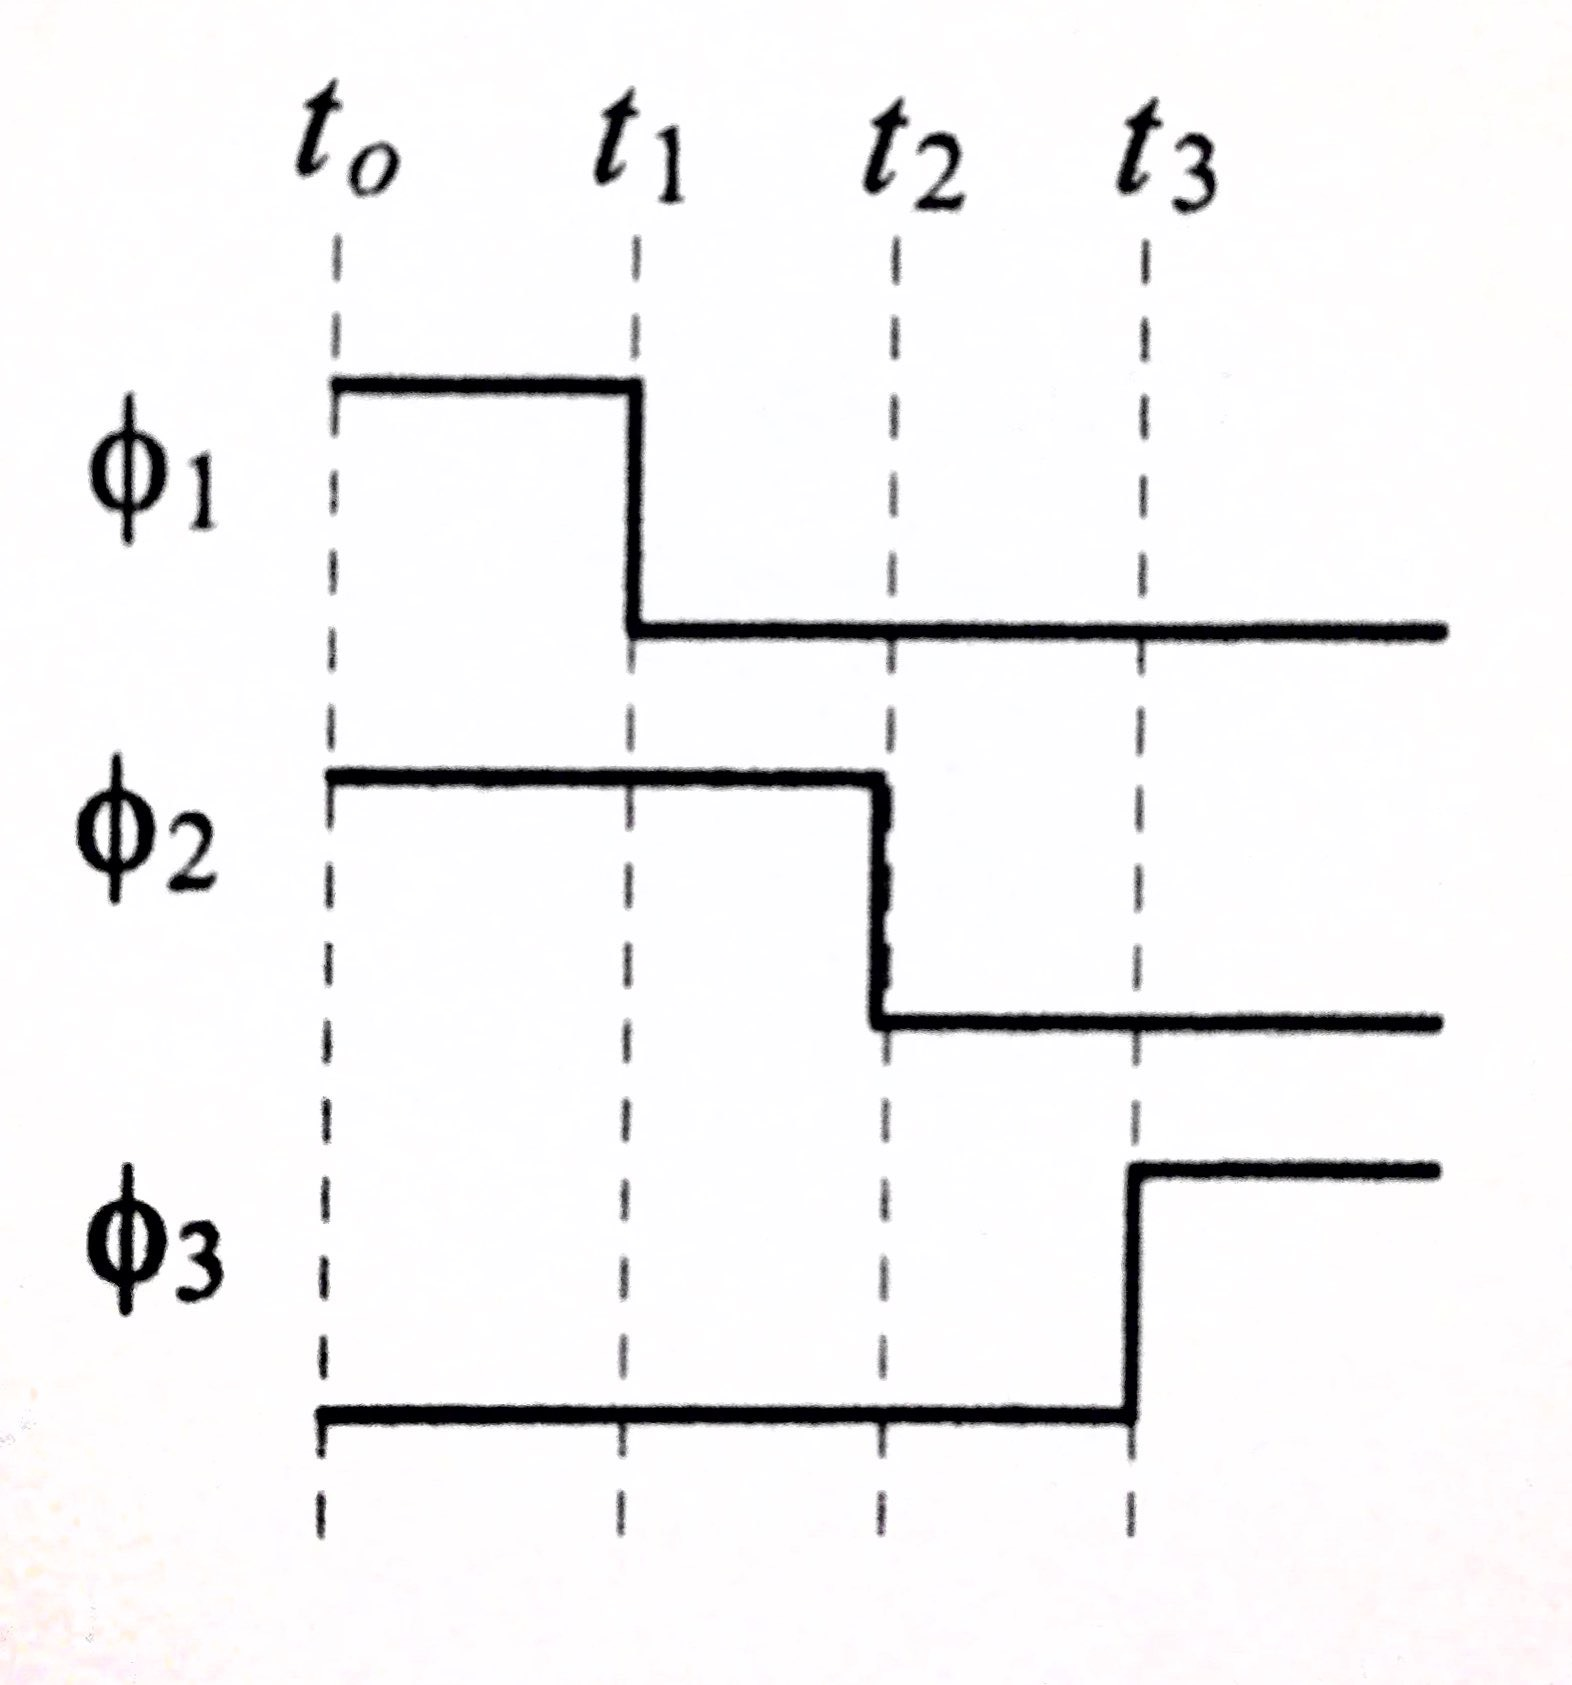
\includegraphics[width=0.4\textwidth]{img/timing_sample_hold.jpg}
   \caption{Single-ended S/H opartion \cite{CMOS-baker}}
   \label{timing}
\end{figure}

%\printbibliography{}
\end{document}
